\section{Implementation}

% Overview
We demonstrate TeleCP, a simple software framework of 3D telepresence. The project is open-source [xx]. Combined with commercial hardware (\$7000 for the two ends), researchers can easily deploy it as a 3D telepresence system. The framework also contains a plugin of Unity3D (an game engine) for easy upper-layer application development. The framework meets our design goal of a high level of co-presence, i.e., the end-to-end delay is 50 ms, sync assistance, shared space and shared props are also supported.

The first several subsections below are for the necessary explanation of the 3D telepresence system. The last subsection introduces how the system supports our design goals.

%Eecach s suwe suppbelois for the necessary w bstionside: CPU $400; GPU $700; network card $400; RAM $200; Disk $200; HTC Vive $1200; Realsense $150*3.

% We demonstrate a lightweight 3DTI system that can be easily deployed by HCI researchers. The system is inexpensive and easy to deploy. The price of equipment is about \$ 7000 for two ends. The project is open-source [xx]. We provide a plugin of Unity3D (an game engine) for easy application development. On the other hand, the system meets our design goal of a high level of co-presence. HMDs provide rich visual information for the system. The end-to-end delay is 50 ms. \emph{Spatial co-presence} and \emph{shared props} are also supported.

\subsection{Hardware requirement and Software Overview}

In summary, a 3DTI system requires reconstruction, transmission and rendering \cite{fuchs2014immersive}. We used TSDF Volume \cite{curless1996volumetric} and Marching Cubes \cite{lorensen1987marching} for reconstruction, a 10 Gigabit Ethernet connection for transmission, and Unity3D for rendering in HTC Vive.

\subsubsection{Hardware}

The system consists of two capture sites in the two distributed rooms. At each capture site, we had three depth cameras for capturing, a PC for computing and an HMD for rendering. Realsense D415 (depth cameras) were used to capture a volume of $2m \times 2m \times 2m$. The locating place of each camera and its contribution to 3D mesh were illustrated in Figure \ref{camera_config}. Each PC had an Intel i7-7700k CPU and a GTX 1080Ti GPU. HTC Vive was used to present the fused reconstruction of both sides. Ten Gigabit network cards (Intel X520-SR2) were used to connect the two capture sites. 

\begin{figure}[!htbp]
\centering
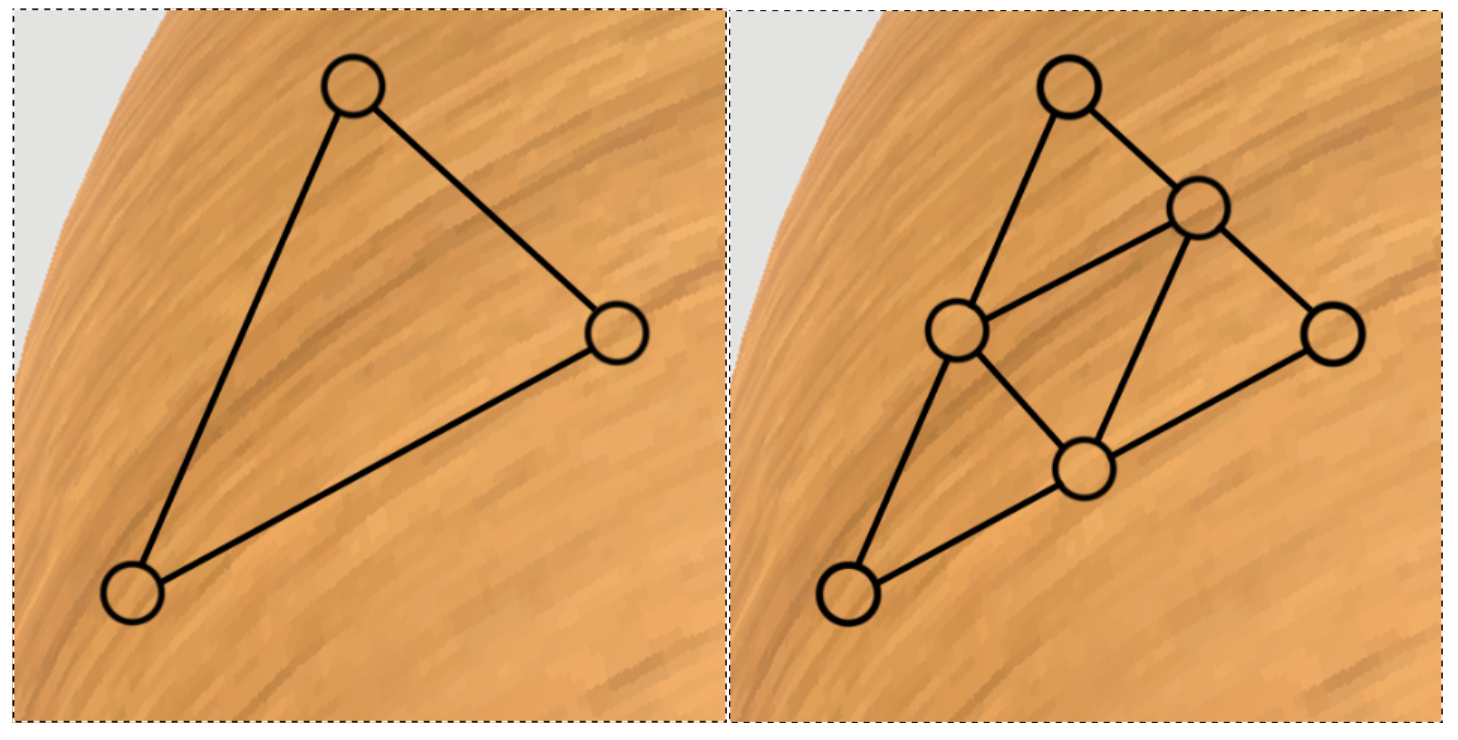
\includegraphics[width=0.9\linewidth]{figures/figure_mc.png}
\caption{The cameras configuration of our system. The different colors of point clouds shows the view of every cameras.}
\label{fig:camera_config}
\end{figure}

\subsubsection{Software}

OpenCV was used for camera calibration. CUDA was used for image processing and the kernel algorithm. Unity3D was used to implement the high-level application. It fetched live reconstruction from the kernel and rendered it in HTC Vive. Python was used for audio transmission.

\subsection{Calibration}

\subsubsection{Calibration between Cameras}

The \emph{camera calibration module} in OpenCV was used to calibrate the cameras. Each pair of cameras took ten snapshots (1080p color images) of a glass-made flat checkerboard. Then, OpenCV aligned their coordinates ($SD < 1 pixel$).

\subsubsection{Calibration between HMD and Cameras}

The HTC Vive was calibrated by setting the original point in its software. We placed the original point of the camera coordinates at the same position by using the checkerboard. Hence, we aligned the HTC Vive with the cameras. This calibration is not necessarily accurate because the users can hardly perceive the error [xx].

\subsection{Preprocessing}

\subsubsection{Depth Processing}

The cameras acquired depth images of $640 \times 480$ pixels at 30 FPS. The Realsense D415 is based on binocular disparity. Thus, disparity values (instead of depth values) were used in the processing for accuracy. We applied median filtering, spatial filtering, hole filling and temporary filtering on the depth images.

\subsubsection{Color Processing}

The cameras acquired color images of $960 \times 540$ pixels at 30 FPS. The exposure settings were manually adjusted. We used one RGB camera as the reference and matched the other cameras to this reference by white balancing and linear mapping.

\subsubsection{Background Removal}

The system can remove unnecessary background and retain only the individuals and the task objects. In the calibration step, we recorded the background as RGBD images. At runtime, we removed pixels that are similar to the background based on thresholds.

\subsection{3D Reconstruction}

We developed a real-time CUDA implementation of 3D reconstruction similar to KinectFusion \cite{izadi2011kinectfusion}. First, the algorithm integrated depth images into a TSDF Volume \cite{curless1996volumetric}. Next, the 3D mesh was extracted from the TSDF Volume using Marching Cubes \cite{lorensen1987marching}. Then, the algorithm projected color images on the 3D mesh for colorization.

The resolution of TSDF volume was $256 \times 256 \times 256$ voxels. In the TSDF processing, we used a weighted average where $W = \frac{1}{Dist}$ on different cameras to minimize the error. In the colorization, each triangle was upsampled to four quartered parts to sample more colors, because the users are more sensitive to the texture but not the shape \cite{sander2001texture}.

\subsection{The support of co-presence}

\subsubsection{Low network delay}

Figure \ref{fig:system_delay} shows the pipeline of our system. The one-way end-to-end delay was 52 ($\pm$ xx) ms, i.e., the time interval between a user acts and his partner sees. The frame rate of 3D reconstruction was 30 FPS. It was restricted by the frequency of Realsense. On average, a frame (33 ms) consisted of 19 ms processing and 14 ms idling. The remote images had one frame of latency. So the end-to-end delay was about $33 + 19 = 52$ ms. The rendering and the audio transmission were independent to the reconstruction pipeline. The frame rate of rendering reached 90 FPS so that the users do not feel dizzy. The audio channel was synchronized with the video channel by appending extra latency.

\begin{figure}[!htbp]
\centering
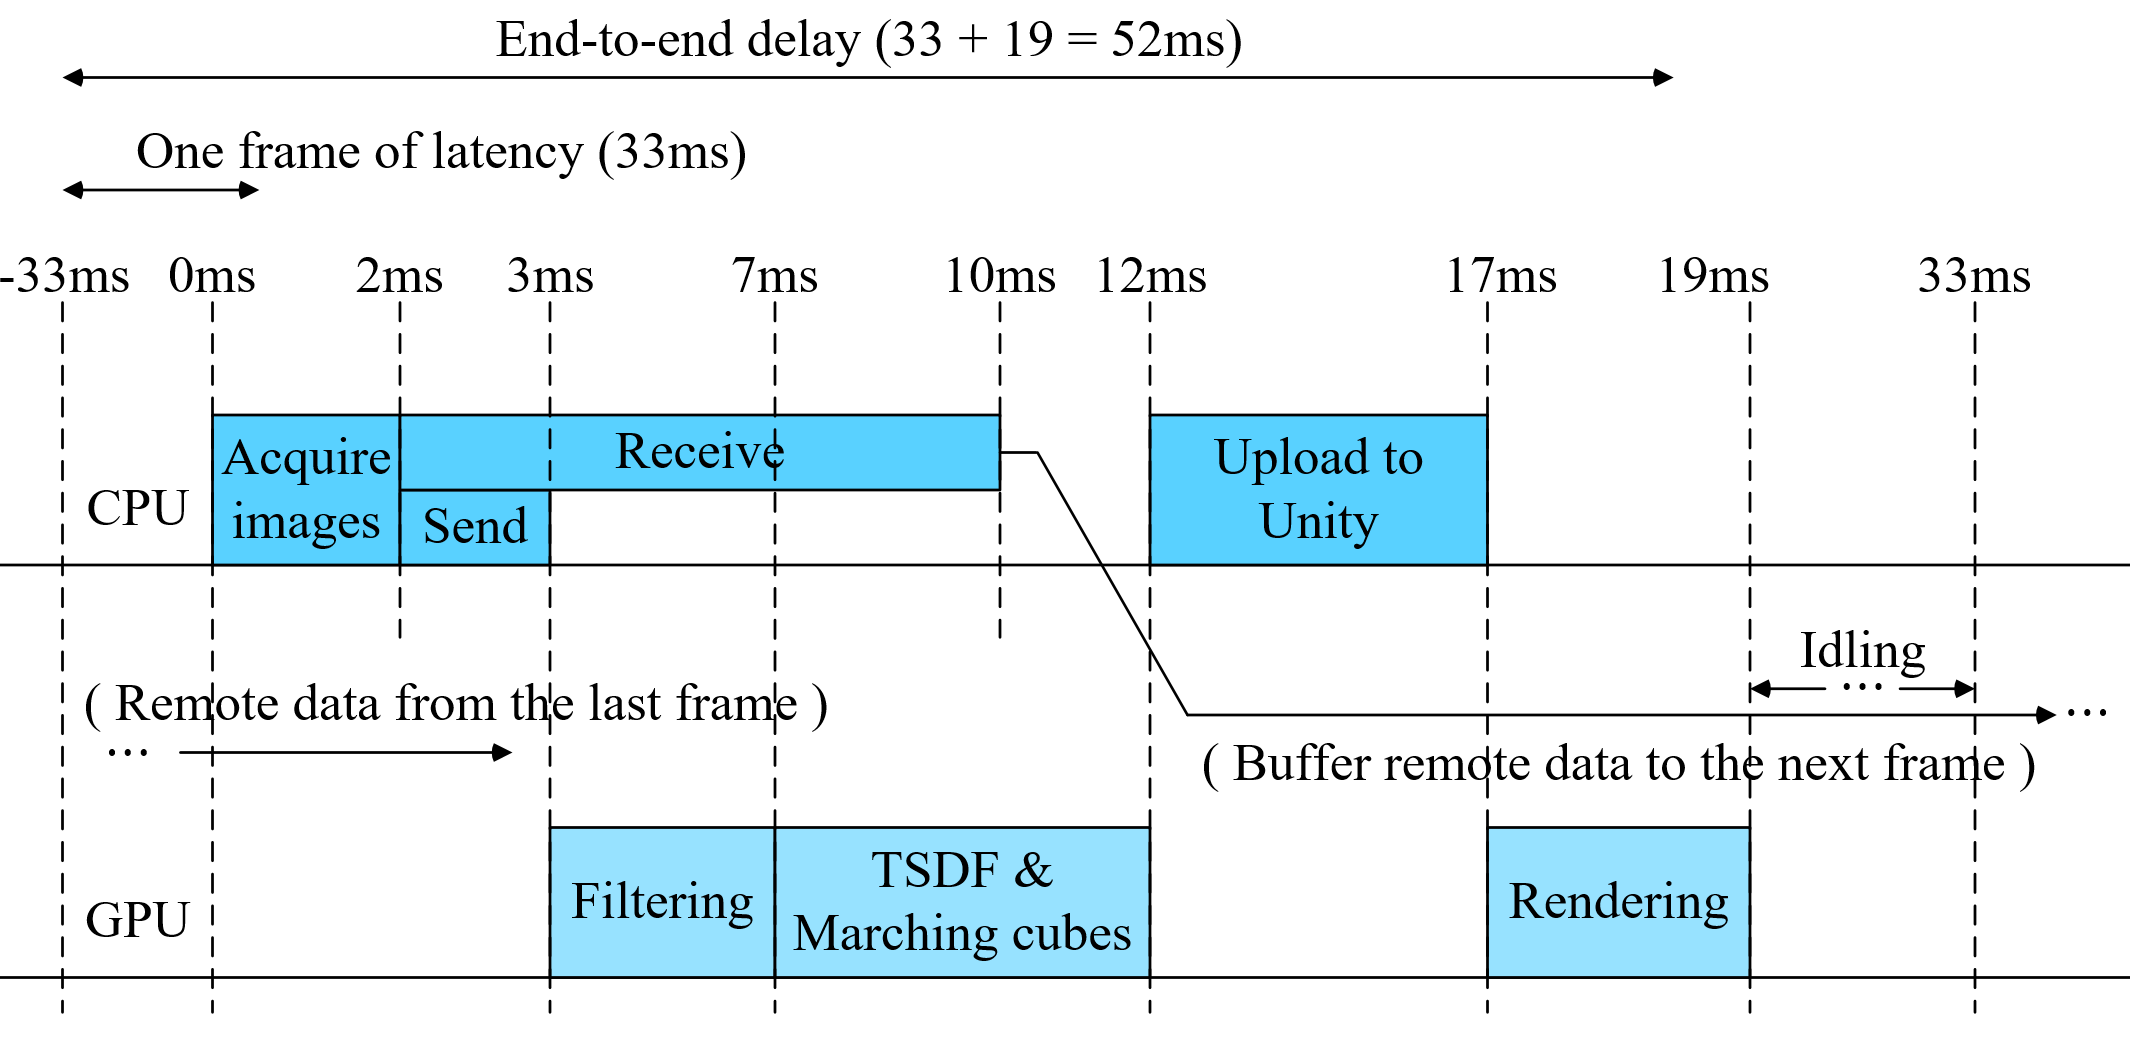
\includegraphics[width=1.0\linewidth]{figures/figure_pipeline_new3.png}
\caption{The pipeline.}
\label{fig:system_delay}
\end{figure}

We reached the high synchronicity by appropriate hardware, efficient GPU implementation and the only one frame of latency. The bottleneck of our pipeline is that Realsense limits a frame to be 33 ms. Another problem is that additional time is wasted in copying data to Unity3D. While Unity3D is important for the easy development, it only receives data through CPU codes, which wastes 5 ms per frame. This problem is possible to be refined in the future.

\subsubsection{Sync assistance}

For the tasks with a very high synchronicity requirement, we propose an assistant design to help synchronizing the task. While the transmission delay of data is unavoidable, it is possible to synchronize the time of two systems with almost zero milliseconds apart (the NTP protocol \cite{mills1991internet}). Thus, it is possible to provide zero-delay cues for the users in the two ends.

Take the Rock-Paper-Scissors game as example, we designed an audio source of "tick, tick, tack". The audio sources are played simultaneously in the two ends. The two users can show the gesture when they hear the "tack" sound. We assessed the effect of this design on user experience in the experiment.

\subsubsection{Shared space}

The system reconstructs physical scene in full 3D and renders it in head-mounted displays. It naturally supports that multiple users feel like locating at the same space.

\subsubsection{Shared props}

For two similar objects from the two ends, our system fuse their common parts together and retain their distinct parts. To create a shared prop, we first map their locations. If the scene contains only one shared prop, we can simply set the location of each physical prop as the origin point of each end. Otherwise we have to move the props to the same location in the virtual space manually. Then, our system merges the shared props automatically.

We modified the TSDF algorithm to merge the shared props. The merging rule is (see more information in \cite{curless1996volumetric}):
\begin{equation}
V_z=\min\{\frac{\sum_{local} W_{i,z}S_{i,z}}{\sum_{local} W_{i,z}},\frac{\sum_{remote} W_{j,z}S_{j,z}}{\sum_{remote} W_{j,z}}\}
\end{equation}
\begin{equation}
W_{i,z}=\frac{1}{dist(i,z)}    
\end{equation}
where $S_{i,z}$ is the Signed Distance Function (SDF) value of the $z$th volume from the $i$th camera. $dist(i,z)$ is the distance from the $i$th camera to the $z$th volume. $V_z$ is the merged SDF value of $z$th volume after the combination.

\begin{figure}[!htbp]
\centering
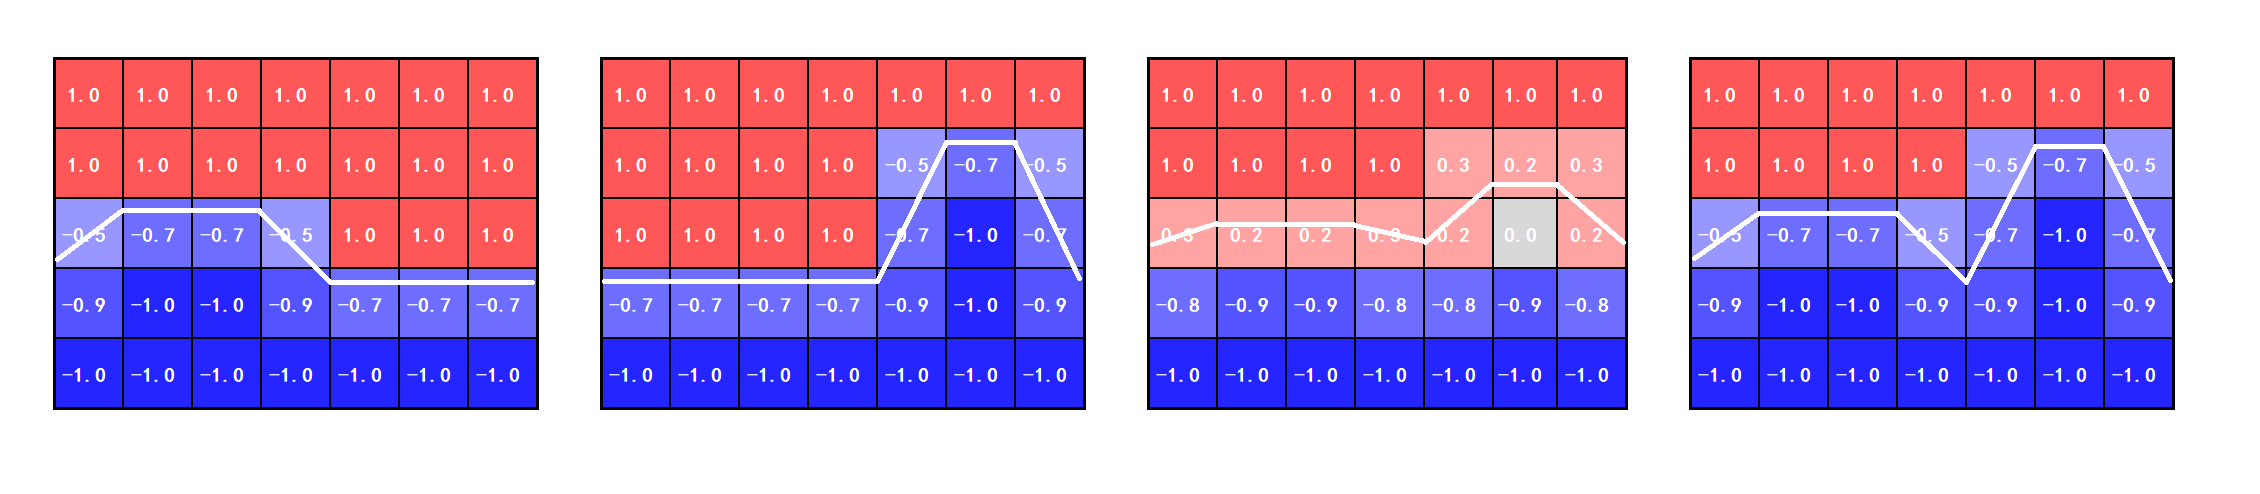
\includegraphics[width=1.0\linewidth]{figures/figure_tsdf.png}
\caption{Left to right: (1 \& 2) SDF values from cameras in the two ends 1; (3) Merged SDF value in a standard TSDF method; (4) Merged SDF value in our framework.【周诚驰】改进merge算法以后,拍两张只有黑棋和只有白棋的特写,再截一张效果图。}
\label{fig:TSDF_merge_two_sides}
\end{figure}

Figure \ref{fig:TSDF_merge_two_sides} shows the weighted combination of the two profile from both ends.
